\documentclass{article}
\usepackage{graphicx}
\usepackage[margin=1.5cm]{geometry}
\usepackage{amsmath}

\begin{document}
\twocolumn

\title{Monday Warm Up: Electrostatics I and II}
\author{Prof. Jordan C. Hanson}

\maketitle

\section{Memory Bank}

\begin{itemize}
\item \textbf{Couloumb's Law}: Let two charges with magnitudes $q_1$ and $q_2$ be separated by a displacement $\vec{r}$.  The force between them is 
\begin{equation}
\vec{F} = \frac{k q_1 q_2}{r^2}\hat{r}
\end{equation}
The vector $\hat{r}$ is a unit vector in the direction of $\vec{r}$, and $r$ is the magnitude.  The constant $k$ is $k=8.988 \times 10^9$ N m$^2$ C$^{-1}$.
\item $\vec{F} = q\vec{E}$ ... The electric field $\vec{E}$ causes the Coulomb force on a charge $q$.
\item \textbf{Couloumb Field}: Let a charge with magnitude $q$ be separated by a displacement $\vec{r}$ from a \textit{test charge}.  The E-field generated by $q$ is 
\begin{equation}
\vec{E} = \frac{k q}{r^2}\hat{r}
\end{equation}
The vector $\hat{r}$ is a unit vector in the direction of $\vec{r}$, and $r$ is the magnitude.  The constant $k$ is $k=8.988 \times 10^9$ N m$^2$ C$^{-1}$.
\item \textbf{Voltage:} Let the negative change in \textbf{voltage}, $\Delta V$, with respect to distance, be equal to the electric field:
\begin{equation}
E = - \frac{\Delta V}{\Delta x} ~\rightarrow~ \vec{E} = -\nabla V
\end{equation}
\item \textbf{Couloumb voltage}: Let a charge with magnitude $q$ be separated by a displacement $\vec{r}$ from a \textit{test charge}.  The voltage generated by $q$ is 
\begin{equation}
V(r) = \frac{k q}{r}
\end{equation}
The constant $k$ is $k=8.988 \times 10^9$ N m$^2$ C$^{-1}$.
\end{itemize}

\section{Electrostatics I and II}

\begin{enumerate}
\item A simple technique for accelerating electrons is shown in Fig. \ref{fig:1} (left).  A uniform E-field is between two plates. Electrons are released from a hot filament near the negative plate. (a) Calculate the acceleration of the electron if the field strength is $2.5 \times 10^4$ N C$^{-1}$. (b) Assume that when the electron leaves the capacitor, it stops accelerating.  If the capacitor is 1 cm wide, and the electron was released from rest, what is the final velocity? (c) What is the final kinetic energy? \\ \vspace{3cm}
\item The classic Millikan oil drop experiment was the first to obtain an accurate measurement of the charge on an electron. In it, oil drops were suspended against the gravitational force by a vertical electric field (Fig. \ref{fig:1}, right).  Given the oil drop to be 1 $\mu$m in radius, and have a density of 920 kg m$^{-3}$.  (a) Find the weight of the drop. (b) If the drop has a charge equivalent to 10 electrons, find the electric field strength needed to balance its weight. \\ \vspace{3cm}
\item (a) If the capacitor in Fig. \ref{fig:1} (left) is 1 cm wide, what is the voltage on it? (b) If the capacitor in Fig. \ref{fig:1} (right) is 5 cm wide, what is the voltage? (c) What is the voltage a distance 1 m from a -1 nC charge?
\end{enumerate}

\begin{figure}
\centering
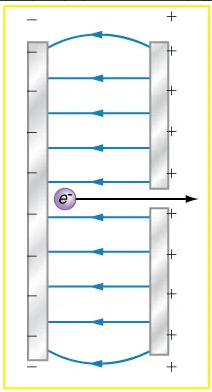
\includegraphics[width=0.175\textwidth]{figures/acceleration.png}
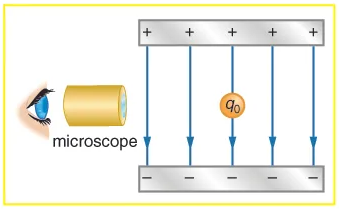
\includegraphics[width=0.225\textwidth]{figures/milliken.png}
\caption{\label{fig:1} (Left) A parallel plate capacitor accelerates an electron. (Right) Idealized Milliken oil drop experiment.}
\end{figure}

\end{document}
